\begin{exo}[... et des carrés]
	On considère le carré $ABCD$ de côtés $6\text{ cm}$ et quatre points $M$, $N$, $P$, $Q$ tels que $AM = BN = CP = DQ$

	On admet que $MNPQ$ est un carré et on note $x = BM$

	\begin{center}
		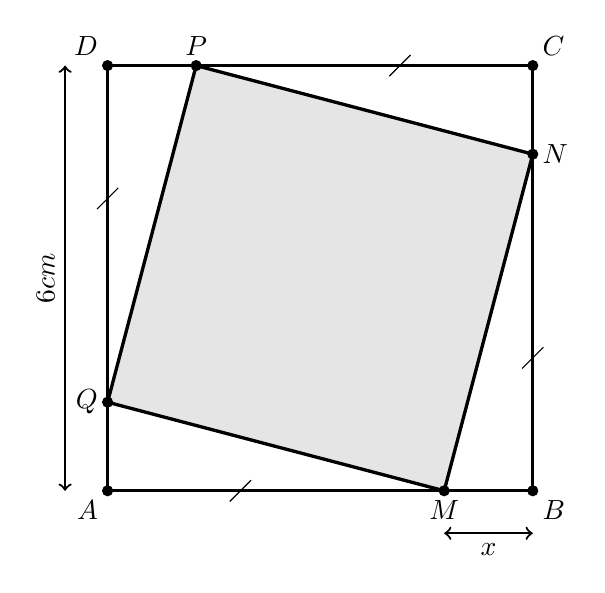
\begin{tikzpicture}[scale=0.9]
			\coordinate (A) at (0,0);
			\coordinate (B) at (6,0);
			\coordinate (C) at (6,6);
			\coordinate (D) at (0,6);
			\draw[very thick] (A) -- (B) -- (C) -- (D) -- cycle;
			\node[below left] at (A) {$A$};
			\node[below right] at (B) {$B$};
			\node[above right] at (C) {$C$};
			\node[above left] at (D) {$D$};
			\coordinate (M) at (4.75,0);
			\coordinate (N) at (6,4.75);
			\coordinate (P) at (1.25,6);
			\coordinate (Q) at (0,1.25);
			\draw[very thick, fill=black!10] (M) -- (N) -- (P) -- (Q) -- cycle;
			\node[below] at (M) {$M$};
			\node[right] at (N) {$N$};
			\node[above] at (P) {$P$};
			\node[left] at (Q) {$Q$};
			\draw[<->, thick] (-0.6,0) -- (-0.6,6) node[midway, above, sloped] {$6\text{ cm}$};
			\draw[<->, thick] (4.75,-0.6) -- (6,-0.6) node[midway, below] {$x$};
			\draw[shift={(1.875,0)}] (-0.15,-0.15) -- (0.15,0.15);
			\draw[shift={(6,1.875)}] (-0.15,-0.15) -- (0.15,0.15);
			\draw[shift={(4.125,6)}] (-0.15,-0.15) -- (0.15,0.15);
			\draw[shift={(0,4.125)}] (-0.15,-0.15) -- (0.15,0.15);
			\foreach \pt in {A,B,C,D,M,N,P,Q} { \filldraw[black] (\pt) circle (2pt); }
		\end{tikzpicture}
	\end{center}

	\begin{enumerate}
		\item Justifier que l'aire $\mathcal{A}$ du carré $MNPQ$ a pour valeur : \cmath{\mathcal{A} = 2x^2 - 12x + 36}
	\end{enumerate}

	\textbf{Aide :} $\text{Aire}(MNPQ) = \text{Aire}(ABCD) - 4 \times \text{Aire}(AMQ)$

	\begin{enumerate}[resume]
		\item \begin{enumerate}
			      \item Montrer que : \cmath{2(x - 2)(x - 4)\ =\ 2x^2 - 12x + 16}
			      \item Déterminer la ou les valeurs de $x$ afin que l'aire du carré $MNPQ$ soit égale aux $\dfrac{5}{9}$ de celle du carré $ABCD$.
		      \end{enumerate}
	\end{enumerate}
\end{exo}
